%\documentclass[3p,twocolumn]{elsarticle}
\documentclass[review]{elsarticle}
\usepackage{graphicx}
\usepackage[export]{adjustbox}%for left right graphic adjust
\usepackage{amsmath}
\usepackage{float}
\usepackage{overpic}
\usepackage{contour}
\usepackage{color}
\graphicspath{ {images/} }

\usepackage[T1]{fontenc}
%\usepackage[utf8]{inputenc}
\usepackage{lineno,hyperref}
\modulolinenumbers[5]

\journal{Journal of \LaTeX\ Templates}

%%%%%%%%%%%%%%%%%%%%%%%
%% Elsevier bibliography styles
%%%%%%%%%%%%%%%%%%%%%%%
%% To change the style, put a % in front of the second line of the current style and
%% remove the % from the second line of the style you would like to use.
%%%%%%%%%%%%%%%%%%%%%%%

%% Numbered
%\bibliographystyle{model1-num-names}

%% Numbered without titles
%\bibliographystyle{model1a-num-names}

%% Harvard
%\bibliographystyle{model2-names.bst}\biboptions{authoryear}

%% Vancouver numbered
%\usepackage{numcompress}\bibliographystyle{model3-num-names}

%% Vancouver name/year
%\usepackage{numcompress}\bibliographystyle{model4-names}\biboptions{authoryear}

%% APA style
%\bibliographystyle{model5-names}\biboptions{authoryear}

%% AMA style
%\usepackage{numcompress}\bibliographystyle{model6-num-names}

%% `Elsevier LaTeX' style
\bibliographystyle{elsarticle-num}
%%%%%%%%%%%%%%%%%%%%%%%

\begin{document}

\begin{frontmatter}

\title{Extending the Dynamic Range of Electronics in a Time Projection Chamber}

%% Group authors per affiliation:
%\author{Elsevier\fnref{myfootnote}}
%\address{Radarweg 29, Amsterdam}
%\fntext[myfootnote]{Since 1880.}

%% or include affiliations in footnotes:
\author[msu,nscl]{J. Estee}
\author[msu,nscl]{W.G. Lynch}
\author[china1,china2]{R. Wang}
\author[msu,nscl]{J. Barney}
\author[msu,nscl]{G. Cerizza}
\author[kor]{B. Hong}
\author[riken]{T. Isobe}
\author[nscl]{G. Jhang}
\author[kyoto]{M. Kaneko}
\author[riken]{M. Kurata-Nishimura}
\author[krakow]{P. Lasko}
\author[kor]{J. W. Lee}
\author[krakow]{J. \L ukasik}
\author[a&m]{A.B. McIntosh}
\author[kyoto]{T. Murakami}
\author[krakow]{P. Paw\l owski}
\author[poland]{K. Pelczar}
\author[nscl]{C. Santamaria}
\author[riken]{D. Suzuki}
\author[nscl]{M. B. Tsang}
\author[a&m]{S.J. Yennello}
\author[tsing]{Y. Zhang}
\author[]{and the S$\pi$RIT collaboration}

\address[msu]{Dept. Physics and Astronomy, Michigan State University, East Lansing, Michigan, 48824, USA }
\address[nscl]{National Superconducting Cyclotron Laboratory, East Lansing, Michigan, 48824, USA}
\address[kor]{Department of Physics, Korea University, Seoul 136-703, Republic of Korea }
\address[riken]{RIKEN Nishina Center, Hirosawa 2-1, Wako, Saitama 351‐0198, Japan }
\address[kyoto]{Department of Physics, Kyoto University, Kita-shirakawa, Kyoto 606-8502, Japan }
\address[krakow]{Institute of Nuclear Physics PAN, ul. Radzikowskiego 15231-342 Krak\'{o}w, Poland}
\address[a&m]{Dept. of Physics and Astronomy, Texas A$\&$M University, College Station, TX 77843, USA }
\address[tsing]{Department of Physics, Tsinghua University, Beijing 100084, P. R. China}
\address[poland]{Faculty of Physics, Astronomy and Applied Computer Science, Jagiellonian University, ul. Go\l \k{e}bia 24, 31-007 Krak\'{o}w}
\address[china1]{State Key Laboratory of Radiation Medicine and Protection, School of Radiation Medicine and Protection, Soochow University, Suzhou 215123, China}
\address[china2]{Collaborative Innovation Center of Radiological Medicine of Jiangsu Higher Education Institutions, Suzhou 215123, China}



\begin{abstract}
As Time Projection Chambers (TPCs) become widely used in low to intermediate nuclear physics experiments,  it becomes important to extend the dynamic range to cover  the large range in energy losses. In a recent set of experiments using the SAMURAI Pion-Reconstruction and Ion-Tracker (S$\pi$RIT) TPC, it was important to simultaneously measure relativistic pions and heavy ions from the same collisions. A track which saturates the TPC electronics only does so for several pads near to the track while pads further away are not saturated. By performing a $\chi^2$ fit using the pad response function on the unsaturated pads, we can recover the saturated pad's charges. This resulted in an increase of the dynamic range by a factor of 5. 
\end{abstract}

\begin{keyword}
\texttt{elsarticle.cls}\sep \LaTeX\sep Elsevier \sep template
\MSC[2010] 00-01\sep  99-00
\end{keyword}

\end{frontmatter}

\linenumbers

\section{Introduction} 
 At low to intermediate heavy ion collision (HIC) energies, one measures particles that have large variations in energy losses ranging from very small energy losses for minimum ionizing particles to much higher energy losses for slower moving complex fragments. This large dynamic range of energy losses presents a problem for the readout of such devices. Finding the solution to this problem has motivated both the development of large dynamic range electronics as well as the development of other methods that can extend the dynamical range of Time Projection Chambers (TPC). In this paper, we discuss and approach that can be applied to expand the dynamic range of existing TPCs.
 
 In principle, readout of these particles could be solved with electronics which are able to switch between high and low gains that cover a very large dynamic range. However, many current TPC's readout electronics have a single gain output with a dynamic range (defined the ratio of the maximum signal to the electronic noise) of no more than 1000:1. In our case the maximum signal to noise was about 400:1. If one sets the electronic gain of such electronics to have a signal to noise ratio for minimum ionizing particles (m.i.p.) of 20:1, then signals that are 20 times larger will be saturated in the electronics. Figure \ref{fig:intro} illustrates the effect saturation has on the measured momentum of the particles. The shaded region shows where 20 times that of the minimum ionizing pion signal where we could expect saturation to occur. While the pion's momentum range can fully be measured without saturation effects, heavier particles would be harder to resolve in dE/dx at lower momentum. 

 Several techniques have been employed to increase the dynamic range for energy losses in TPCs. For example, in the EOS TPC \cite{eos} a larger dynamic range was achieved by lowering the voltage on selected anode wires, thereby decreasing the gas amplification on those wires. In the prototype Active Target TPC (PAT-TPC) and equivalent reduction in gain was achieved by lowering  the electronics gain setting for some of the readout channels. Such schemes achieve increased dynamic range by optimizing the gain for weakly ionizing ions in some section and optimizing the gain of other sections for strongly ionizing ions. 
 
 These strategies have drawbacks because in many applications the experiment's requirements cannot accept the associated degradation in the dE/dx resolution or the momentum resolution. Here we illustrate an alternate approach to expand the dynamic range within the context of a standard multi-wire TPC without the need of extra hardware or dedicating regions of lower gain. 
 
\begin{figure}[H]
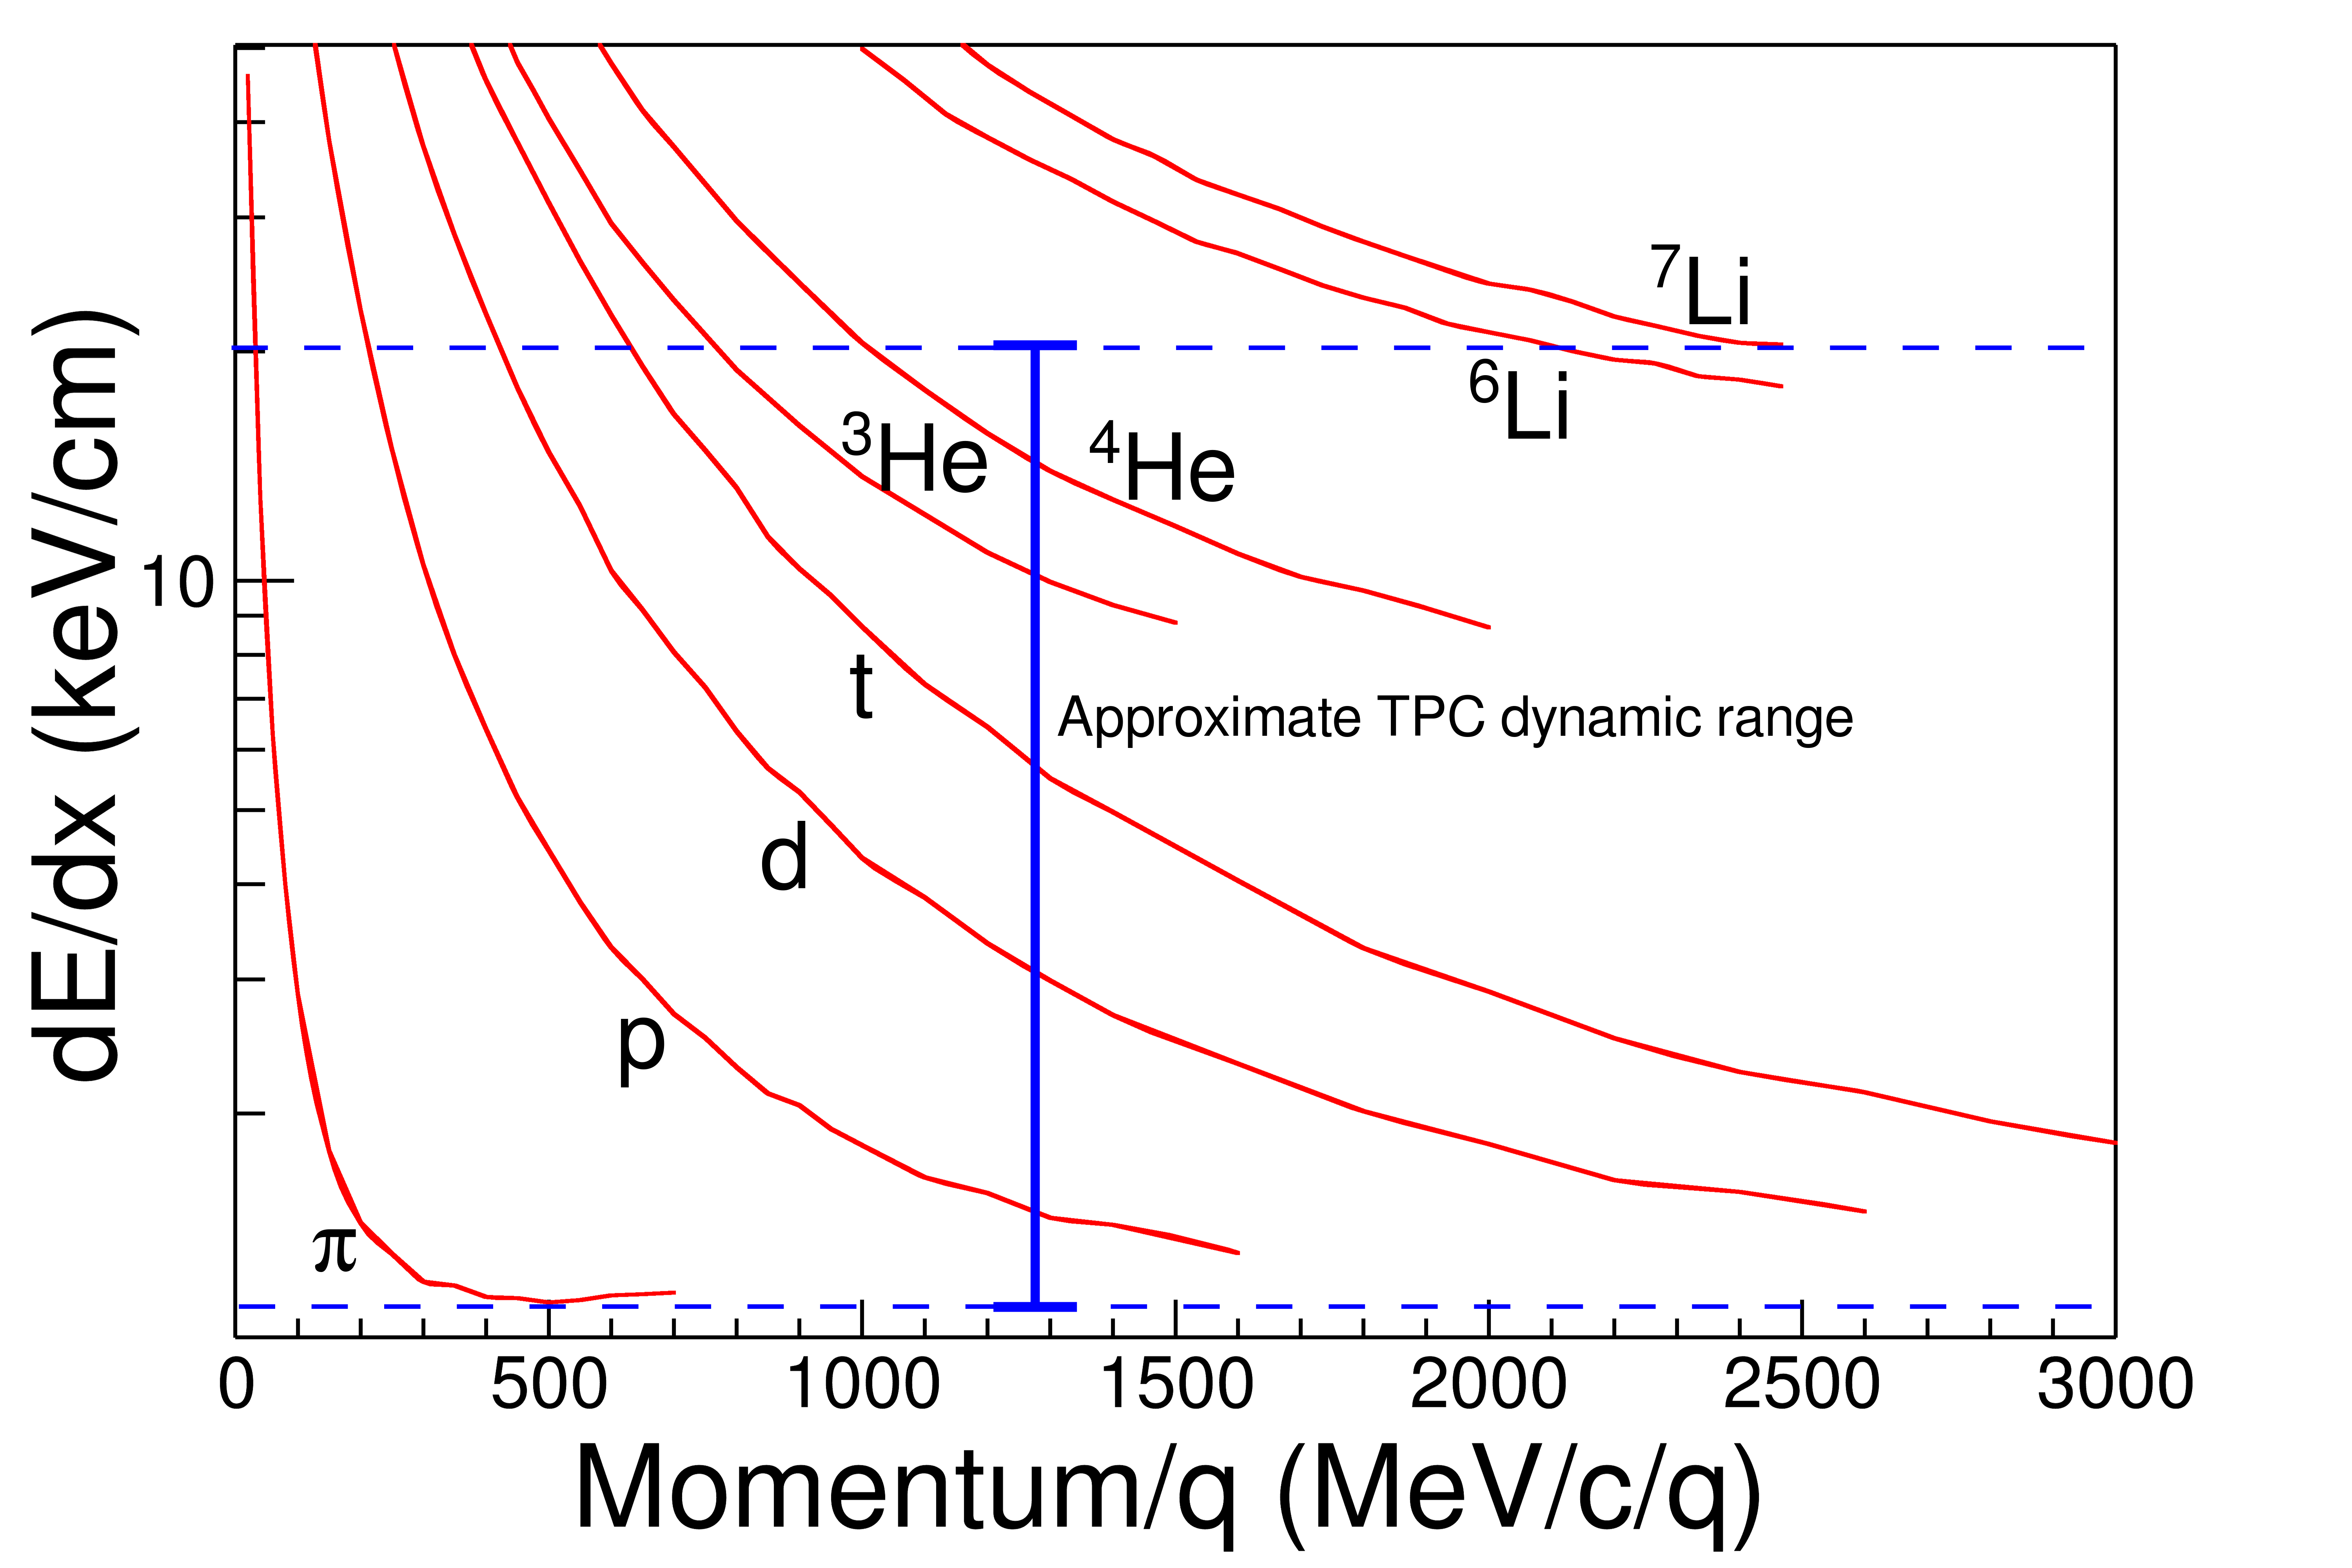
\includegraphics[width=\linewidth]{intrographic}
\caption{}
\label{fig:intro}
\end{figure}

\paragraph{1.1 TPC Overview}
We begin our discussion by describing some basic properties of the SAMURAI Pion Reconstruction and Ion-Tracker (S$\pi$RIT) TPC. For the following discussion we have defined the +x axis to point to the left of beam, the -y axis to point down into the drift volume, and the +z axis to point along the incoming beam. This discussion starts with the wire and pad plane structures of the TPC. 

\begin{figure}[H]
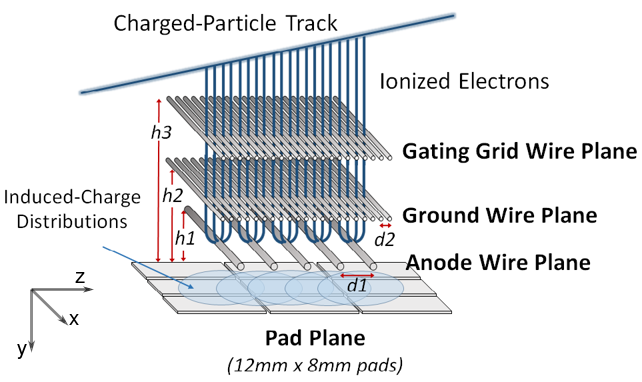
\includegraphics[width=\linewidth]{padwire}
\caption{Cartoon graphic showing the 3 wire planes and a section of the pad plane. h3 =14 mm, h2 = 8 mm, h1 = 4 mm, d2 = 1 mm, d1 = 4 mm. This graphic is inverted from the actual wire planes and pad plane to display the perspective easier.}
\label{fig:padwire}
\end{figure}

\paragraph{Wire planes}
As seen in figure \ref{fig:padwire} the S$\pi$RIT TPC consists of three wire planes below the pad plane which is a two dimensional array of charge sensitive readout pads. The wires are aligned along the x-axis. The first wire plane operates as an ion-gate or gating grid. The second wire plane is held at ground. Both wire planes serve to isolate the drift volume from the gas amplification stage. The wire plane closest to the pad plane is the high voltage anode wire plane consisting of 20 $\mu$m in diameter wires spaced at 4 mm apart and set at a height of 4 mm from the pad plane. In the near vicinity of these wires an avalanche  occurs that multiplies the secondary electrons that drift up from the drift volume. These secondary electrons were created when the track traversed the detector gas in the drift volume. When these secondary electrons reach the anode wires, they are multiplied on the order of 1000 times creating electron and ion pairs. It is the motion of these slow moving ions drifting away from the anode wires that induce images charges on the read out pads above. The distribution of image charge signals on the pad plane is fixed by the geometry of the anode wire grid and its distance from the pad plane. The anode wires were sectioned off into 14 independent sections containing 26 wires; 12 sections were biased to 1460 V. This setting was chosen to ensure  minimum ionizing pions would at have a signal to noise ratio of around 20:1. The two remaining sections were biased to 1214 V due to high current issues, reducing the gas gain by a factor of 10x as compared to the other anode sections. These two sections of lower gain effectively extended the dynamic range. Lowering the anode wires were not necessary for the following but allows for a direct validation of the method that will be described. 

\paragraph{Pad plane} 
The S$\pi$RIT TPC pad plane consists of a 2-dimensional plane of rectangular charge sensitive pads with an x dimension (transverse to the beam) of of 0.8 cm wide and a z dimension of 1.2 cm (along the beam axis). These pads are laid out on a grid measuring 112 by 108 pads with a total area of 134 cm x 86 cm. For convenience we have chosen the +x axis to point to the left of beam, the -y axis as the direction pointing down into the drift volume, and the +z axis along the incoming beam. The anode wires run perpendicular to the beam axis along the x axis as seen in the figure \ref{fig:padwire}. 

\paragraph{Generic Electronics for TPCs}
Signals from the pads in the S$\pi$RIT TPC are amplified and digitized by the recently developed Generic Electronics for TPCs (GET) \cite{get}.  Short cables transmit the signals from the pads to the inputs of the AGET chips. Each AGET chip can service 64 pads and contains a Preamp (PA), and a Switched Capacitor Array (SCA) with a maximum of 512 time buckets sampling at 1 to 100 MHz. Four AGET chips are mounted on one AsAd (ASIC and ADC) motherboard. The gain of each AGET can be configured as 0.12, 0.24, 1.0, or 10 pC over the whole dynamic range. Also the peaking times of the shaping amplifiers can be set to 69, 117, 232, 501, 720, or 1014 ns. The ADCs on the AsAd boards provide 12 bit resolution. In the following, the gain was set to the highest setting, 0.12 pC, the peaking time was 117 ns, and the width of the time bucket was  40 ns. The selected electronics and anode gain setting allowed, the pion signal to be measured while risking saturation for other charged particles. Figure \ref{fig:intro} shows the approximate region which particles experienced saturation for these settings.

\section{Pad Response Function}
\paragraph{Experimental PRF}
When electrons from a track are multiplied on the anode wires, this induces a 2-dimensional image charge distribution on the pad plane. The fractional charge seen by each pad is referred to as the Pad Response Function (PRF). Some simple wire plane geometries have analytical expressions for the PRF that are well studied and may be looked up using a Gatti distribution \cite{blumrol}. When analytic PRFs do not exist, an effective PRF may be calculated from experimental data.  This approach is used here. We postulate that the PRF is only a function of the total charge deposited on the wire Q and the displacement, $\lambda$, from the mean avalanche position $\bar{x}$.

\begin{figure}[H]
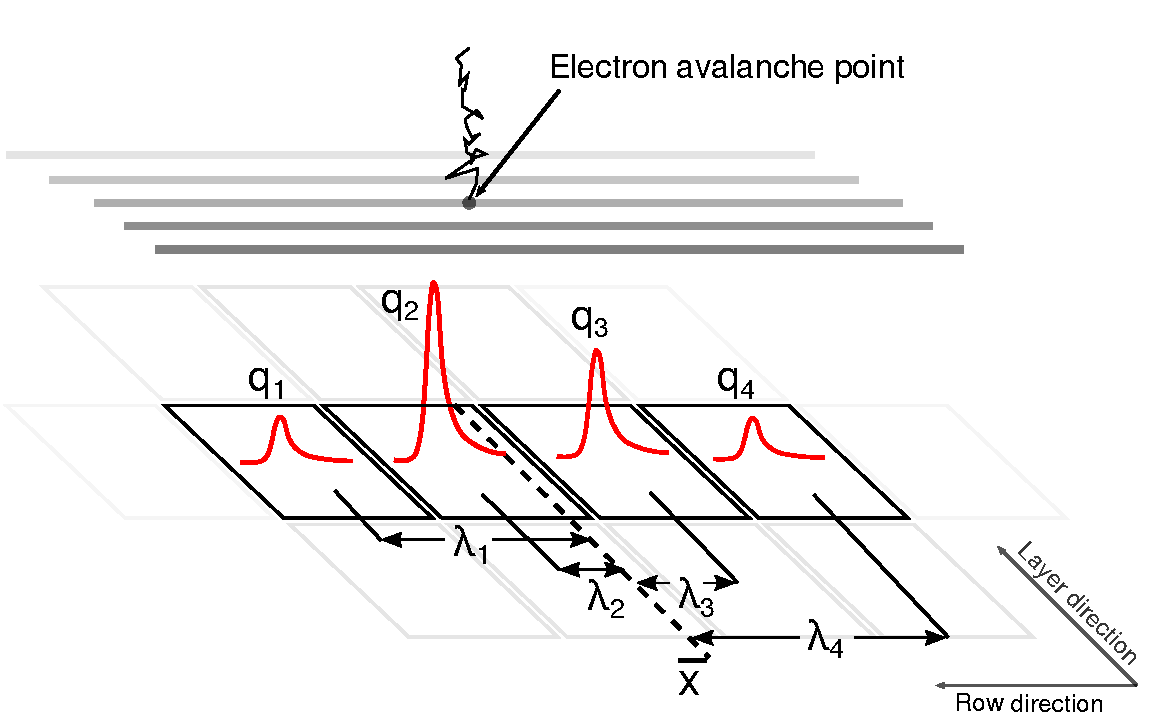
\includegraphics[width=\linewidth]{defofavalanche}
\caption{Cartoon graphic of avalanche event on an anode wire over one layer of pads. The estimate of the position of the avalanche is given by $\bar{x}$  the mean. The position from the center to each pad to the $\bar{x}$ position is given as $\lambda_i$.}
\label{fig:av}
\end{figure}

\begin{equation}\label{eq:1}
\begin{split}
PRF(\lambda_i) = \frac{q_i(\lambda_i)}{Q}\\
where \ Q=\sum_i q_i\\
and \   \lambda_i=x_i-\bar{x}\\
\end{split}
\end{equation}

\begin{equation}\label{eq:gatti}
\begin{split}
PRF_{gatti}(\lambda)
& = \frac{K_{1}}{K_{2}\sqrt{K_{3}}}\bigl[arctan(\sqrt{K_{3}}tanh\bigl[K_{2}\bigl(\frac{x}{h}+\frac{w}{2h}\bigr)\bigr]) \\
& - arctan(\sqrt{K_{3}}tanh\bigl[K_{2}\bigl(\frac{x}{h}-\frac{w}{2h}\bigr)\bigr])\bigr] \\
& K_{1} = \frac{K_{2}\sqrt{K_3}}{4 atan(\sqrt{K_3})}\\
& K_2 = \frac{\pi}{2}\left(1-\frac{\sqrt{K_{3}}}{2}\right)\\
\end{split}
\end{equation}

\begin{equation}\label{eq:gaus}
PRF_{gaus}(\lambda) = .5\left[erf\left(\frac{x+\frac{w}{2}}{\sqrt{2}\sigma}\right) - erf\left(\frac{x-\frac{w}{2}}{\sqrt{2}\sigma}\right) \right]
\end{equation}

For the purpose of calculating the effective PRF from experimental data, we select only the pads that are not saturated. In the full TPC analysis we cluster by layer or by row depending on the angle the track makes with respect to the wire. For the following we only illustrate the layer clustering case but clustering by row follows the exact procedure with a different PRF. 

The way we calculate the PRF is given by equation \ref{eq:1} where i is the index over the pads and Q is the total charge within the layer. Figure \ref{fig:av}  illustrates the estimate for the avalanche position along the wire given by, the mean position $\bar{x}$. Also seen is $\lambda_i$, defined as the difference in position of the center of the $i^{th}$ pad, $x_i$, to the mean position $\bar{x}$. 


\begin{figure}[H]
\begin{overpic}[grid,width=\linewidth]{expprf}
\put(65,55){\contour{white}{\fontsize{5}{6}$\frac{K_{1}}{K_{2}\sqrt{K_{3}}} arctan(\sqrt{K_{3}}tanh\left[(K_{2}(\frac{x}{h}+\frac{w}{2h})\right]) - arctan(\sqrt{K_{3}}tanh\left[(K_{2}(\frac{x}{h}-\frac{w}{2h})\right])$  }}
\put(65,45){\contour{white}{    }}
\end{overpic}
\caption{Experimental pad response function. Constructed from total number of pads $>$=3. }
\label{fig:expprf}
\end{figure}


%\begin{figure}[H]
%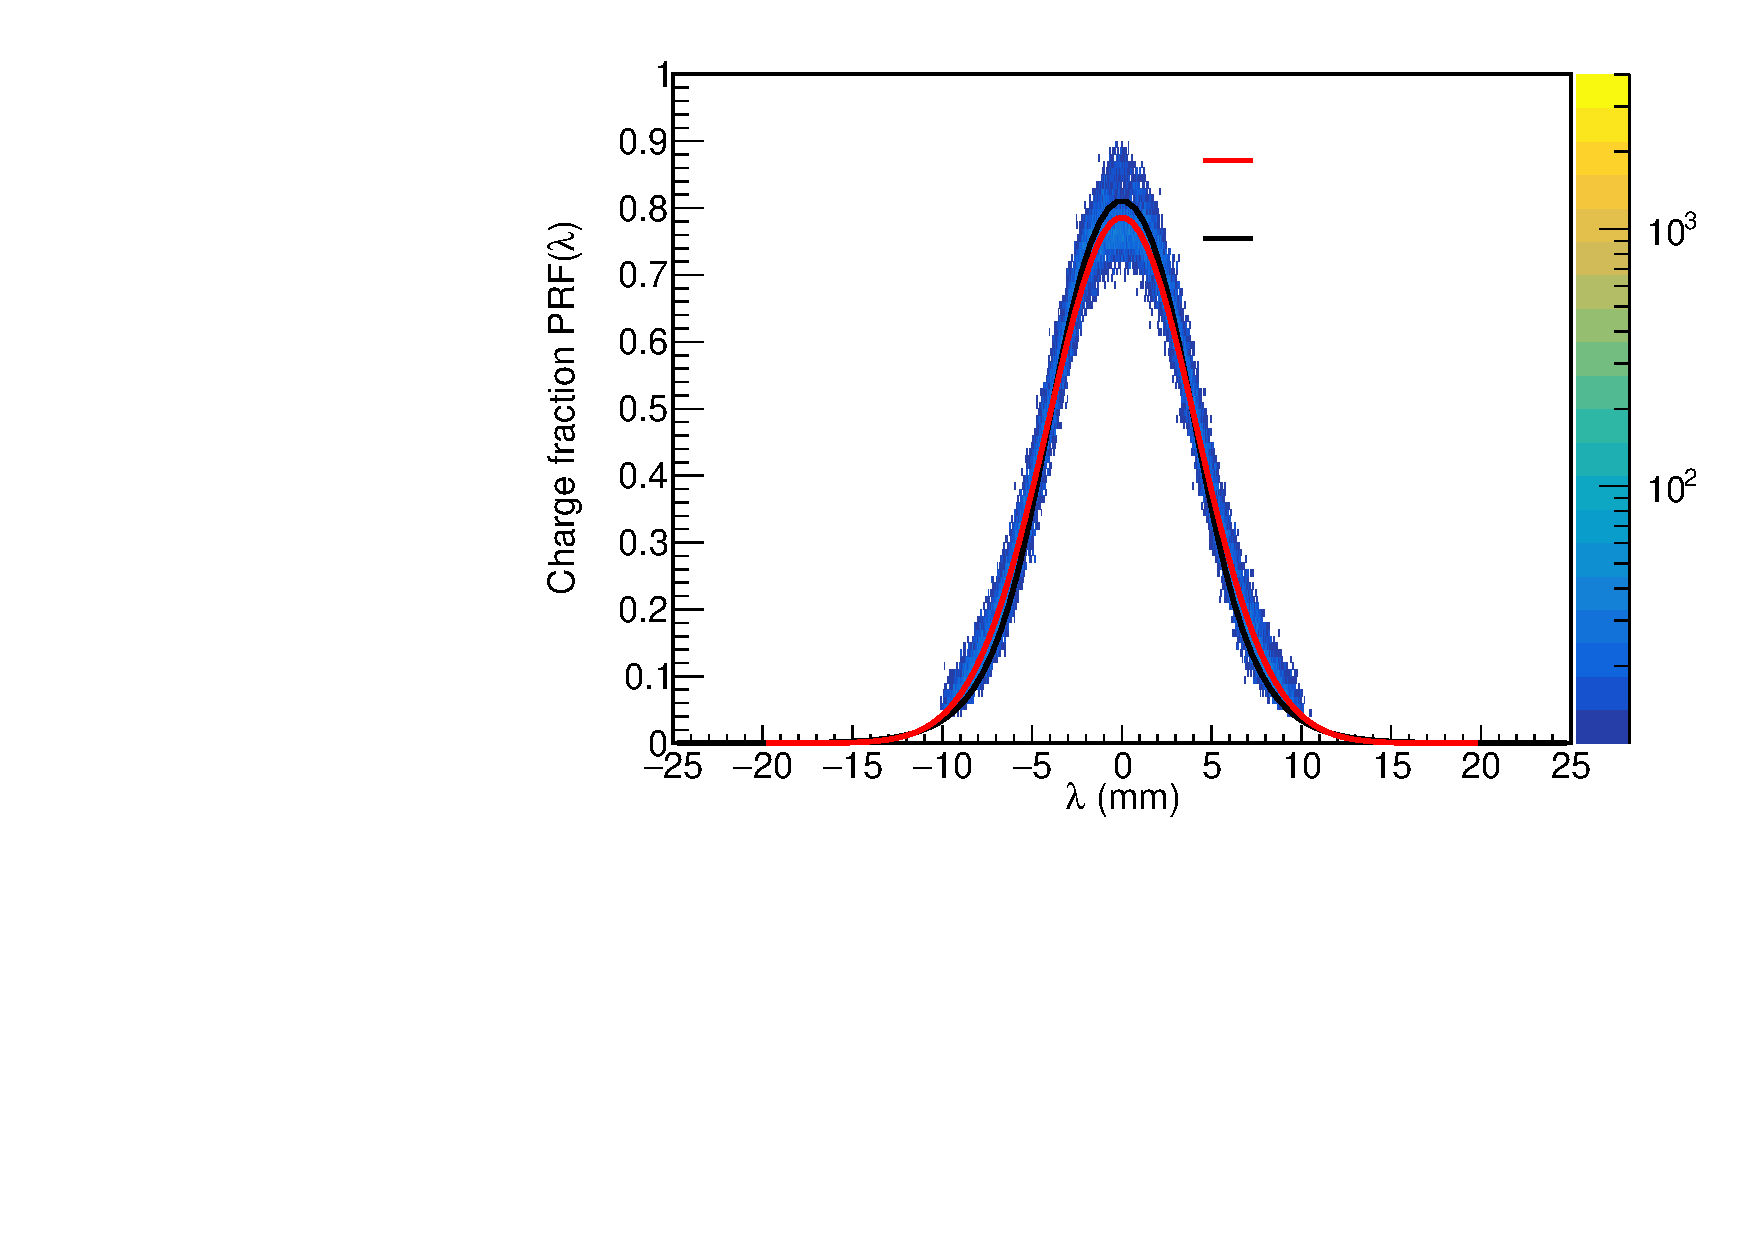
\includegraphics[width=\linewidth]{expprf}
%\caption{Experimental pad response function. Constructed from total number of pads $>$=3. }
%\label{fig:expprf}
%\end{figure}

The resulting experimental PRF for the S$\pi$RIT TPC is shown in figure \ref{fig:expprf}.This well-behaved function is obtained from averaging many events. In the following this function will be used to fit the data and correct for the saturated pads. 
\paragraph{Method of Desaturation}

We will use the term ``desaturation" for our process of estimating and correcting the charge values of the saturated pads. Figure \ref{fig:satpad} shows a typical situation of saturated signals. When an avalanche causes a large induced signal, the pads directly underneath collect the largest charge and may become saturated. We label these charges $q_{2'}$ and $q_{3'}$ as indicated in figure \ref{fig:satpad}. The pads further away would experience smaller, non-saturated signals shown as $q_{1}$ and $q_{4}$.

Since the charge deposited on each  pad must satisfy the PRF distribution described in figure \ref{fig:expprf}, then including these small non-saturated tails in, $q_{1}$ and $q_{4}$, we perform a $\chi^2$ fit to find the unknown charge on the saturated pads. The data points of the $\chi^2$ fit are the unsaturated pads,  $q_{1}$ and $q_{4}$, and the unknown parameters of the fit are $q_{2'}$ and $q_{3'}$ with the expected values coming from the PRF described above. The values of $q_{2'}$ and $q_{3'}$ at the minimum of the $\chi^2$ would be the best estimate for the saturated pads. 
\begin{figure}[H]
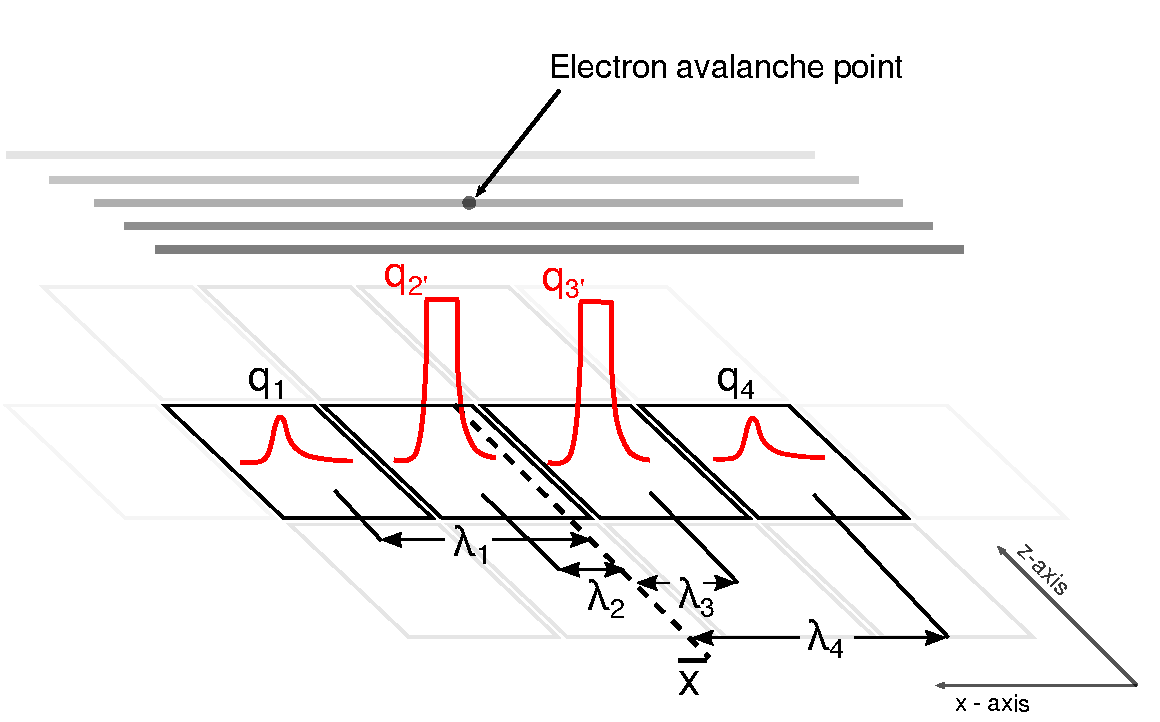
\includegraphics[width=\linewidth]{saturated_pads}
\caption{•}
\label{fig:satpad}
\end{figure}

\section{Experimental data}
Two sets of data were used for the testing and validation of this method. The first set was a tuned cocktail beam consisting of (p,d,t,${}^3He$,${}^4He$,${}^6Li$,${}^7Li$) light charged particles which was injected into the TPC for calibration purposes. The cocktail beam was tuned to two different $\beta\rho$ settings and the momentum resolution was approximately 1\% as determined by the slits of the BigRIPS fragment separator of the Radioactive Isotope Beam Factory (RIBF) facility in RIKEN. A thick 21mm thick aluminum target was inserted for part of the lower $\beta\rho$ setting, further reducing the energy of the beam for a third calibration point. 

In a typical cocktail event one particle enters the TPC volume at a time and mostly parallel to the pad plane. Therefore the cocktail beam data represents an ideal case for the momentum and dE/dx determination as it does not suffer from inefficiencies related to high multiplicity events we see in the collision experimental data.  

\begin{figure}[H]
\includegraphics[width=\linewidth]{data.pdf}
\caption{Pad plane projection for a collision event in the TPC. Highlighted by red arrows are two regions of anode wires which had a reduced voltage of 1214 V. The voltage of the rest of the TPC anode wires are 1460 V. The reduction in voltage reduces the gain by a factor of about 10x. }
\label{fig:data}
\end{figure}

The other type of data was the collision of a ${}^{132}$Sn beam onto a ${}^{124}$Sn target in which we triggered on central nuclear collisions. Shown in figure \ref{fig:data} is the typical pad plane response for a central nuclear collision. During the experiment the voltages of two anode sections (as indicated by red arrows in figure \ref{fig:data}) were biased to 1214 V. Since the anode voltages were dropped, the gain of these sections were also reduced by a factor of about 10x as compared with the other sections which were biased to 1460 V. 


\section{Results}
\paragraph{Low gain vs corrected high gain}

Since these two lower gain sections are lowered in anode voltage the dynamic range as compared with the high gain regions is approximately 10x larger. Tracks which saturate pads in the high gain region are below saturation in the low gain region. By comparing the dE/dx values of the high gain sections with the low gain section we can directly measure whether the desaturation of the high gain region described above is successful. 

\begin{figure}[H]
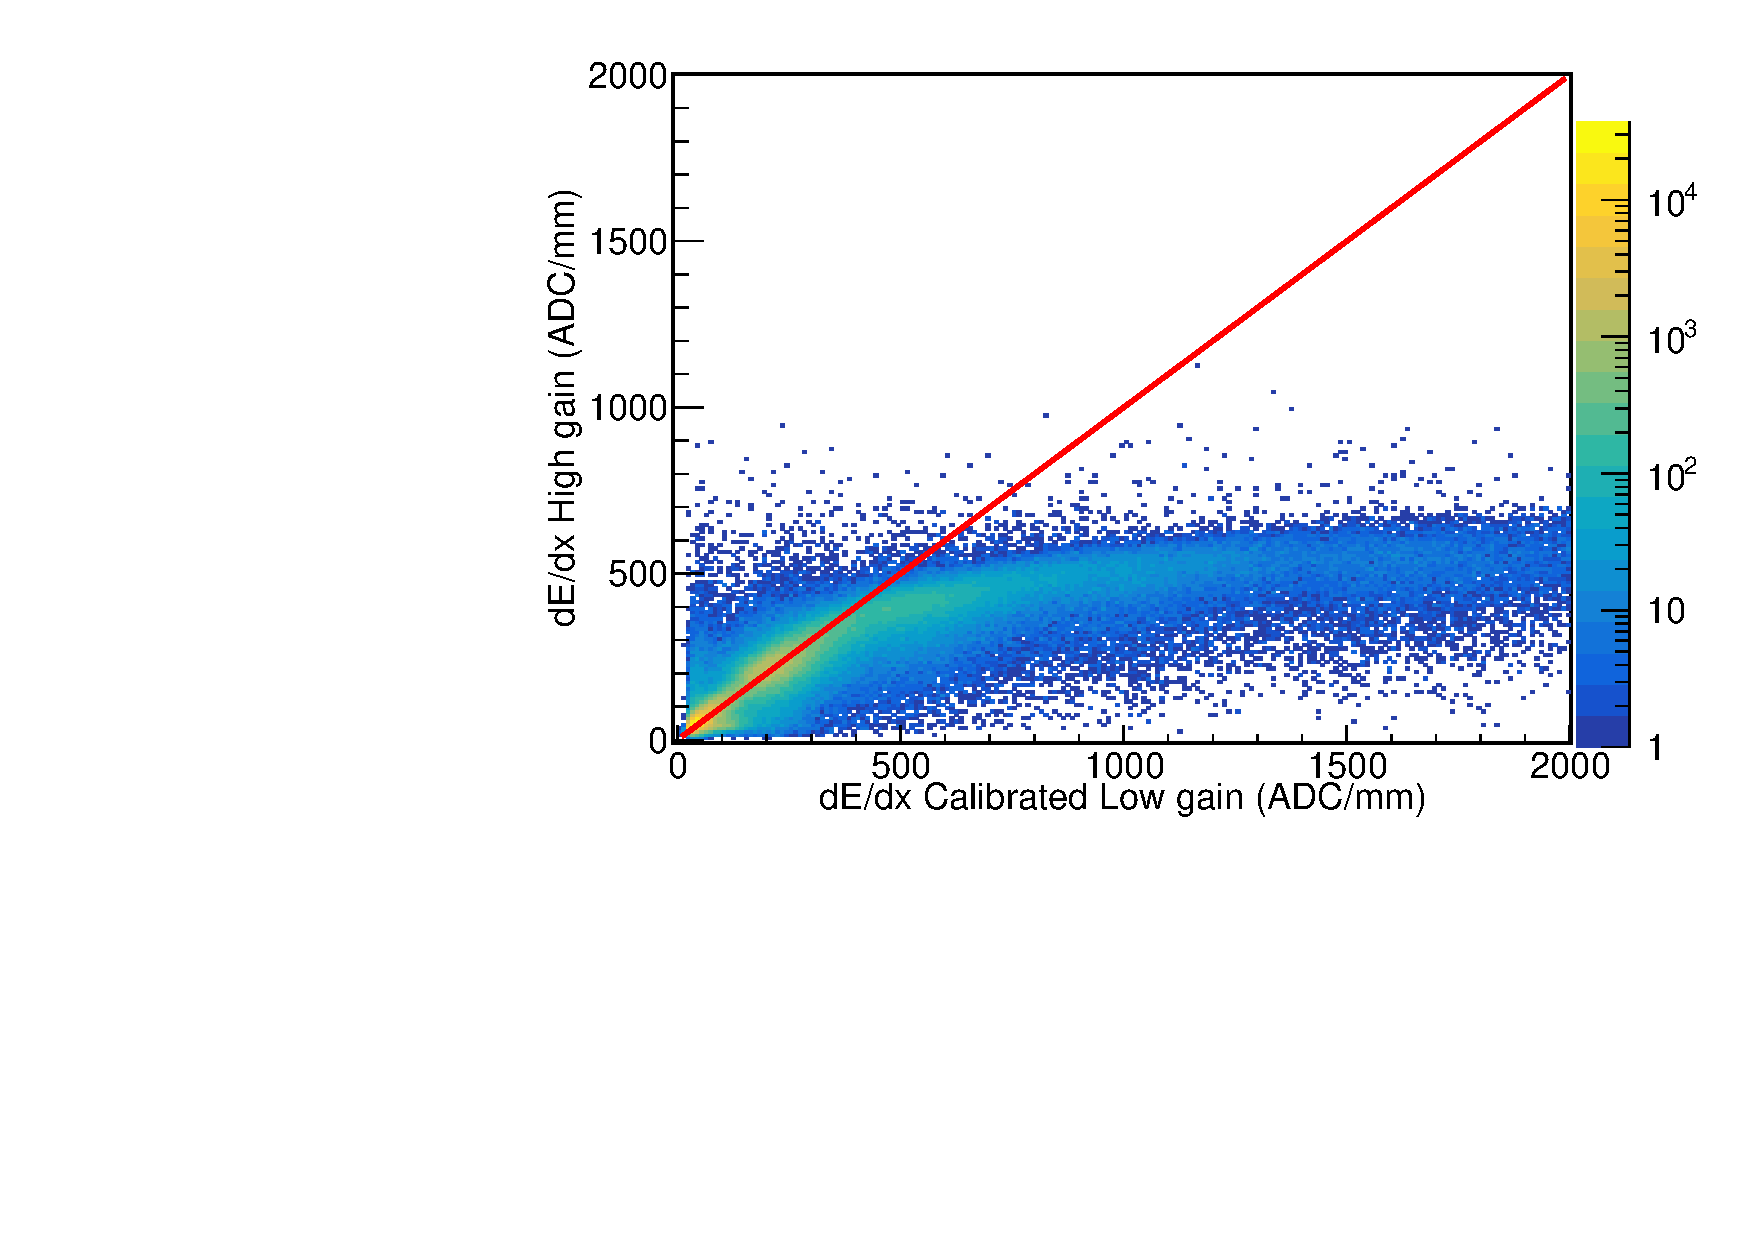
\includegraphics[width=\linewidth]{dedxcompare_nodesat}
\caption{The uncorrected high gain dE/dx vs low gain dE/dx collision data.  }
\label{fig:lowvshigh_raw}
\end{figure}
 
Plotting the uncorrected data in figure \ref{fig:lowvshigh_raw}, the effect of saturation can be seen on the high gain channels. For signals in size below 400 ADC/mm the electronics are not saturated and therefore the high and low gain sections agree. The data starts to saturate and deviates above 400 ADC/mm in the high gain channels and eventually reaching a plateau. Though these events saturate the high gain sections the low gain sections still have not saturated and provide true dE/dx values. After applying the desaturation method, the correlation between the high gain and low gain sections is restored as seen in figure \ref{fig:lowvshigh_desat}. Judging by the data in the corrected correlation plot we believe the correction to at least about 2000 ADC/mm. It seems the 1:1 correlation, which was a plateau before, is restored and an increase in dynamic range by at least a factor of 5x.  

\begin{figure}[H]
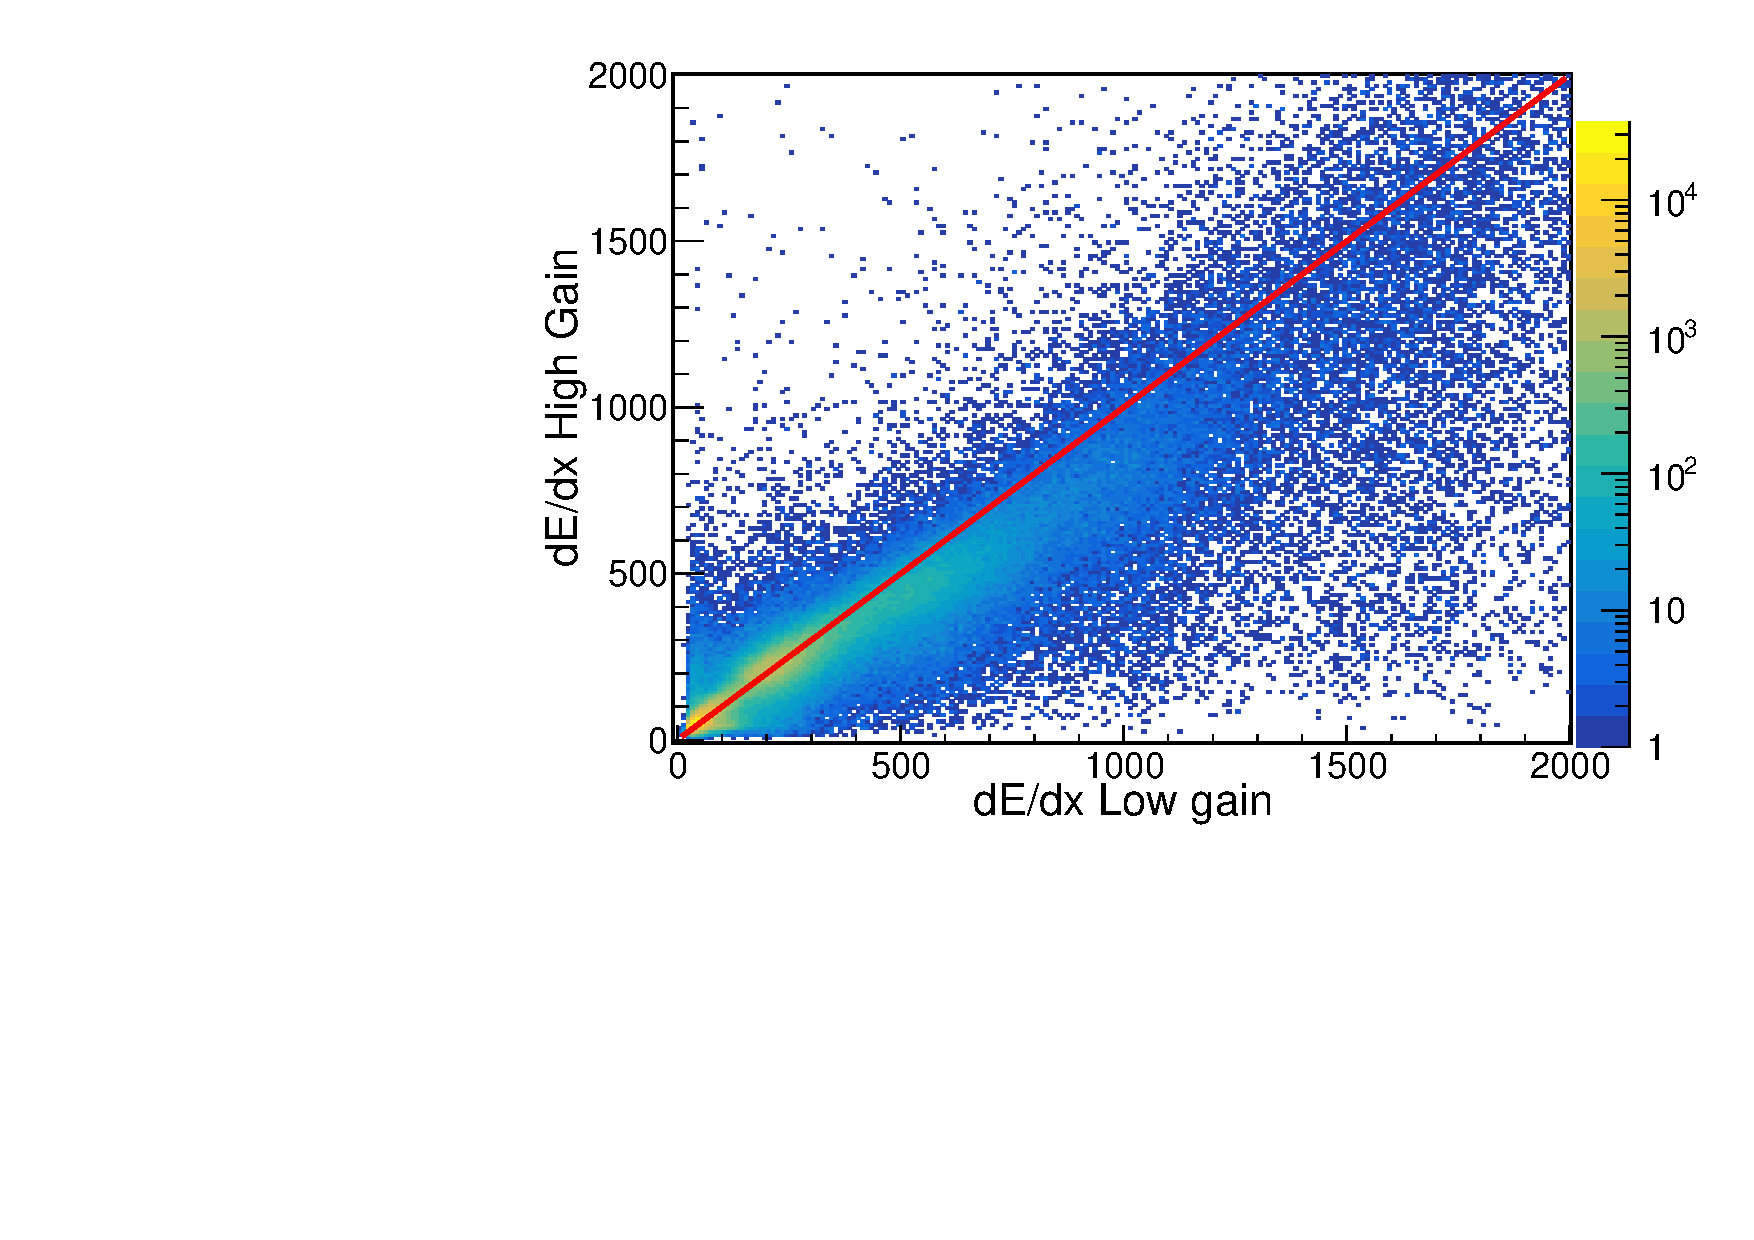
\includegraphics[width=\linewidth]{dedxcompare_new}
\caption{The corrected high gain dE/dx vs low gain dE/dx for collision data.  }
\label{fig:lowvshigh_desat}
\end{figure}

\paragraph{Particle Identification (PID)}

Comparing the low to high gain sections provides a direct measurement for determining the success of the desaturation technique but, the goal would be to improve the particle identification (PID). 

\begin{figure}[H]
\begin{overpic}[width=\linewidth]{cocktail_sat.png}
\put(22,15){\contour{white}{\Large p} }
\put(27,20){\contour{white}{\Large d} }the
\put(31,25){\contour{white}{\Large t} }
\put(30,31){\contour{white}{\large ${}^{3}$He} }
\put(33,35){\contour{white}{\large ${}^{4}$He} }
\put(60,27){\contour{white}{\large ${}^{6}$Li} }
\end{overpic}
\caption{Uncorrected cocktail data.}
\label{fig:cocktail_raw}
\end{figure}

%\begin{figure}[H]
%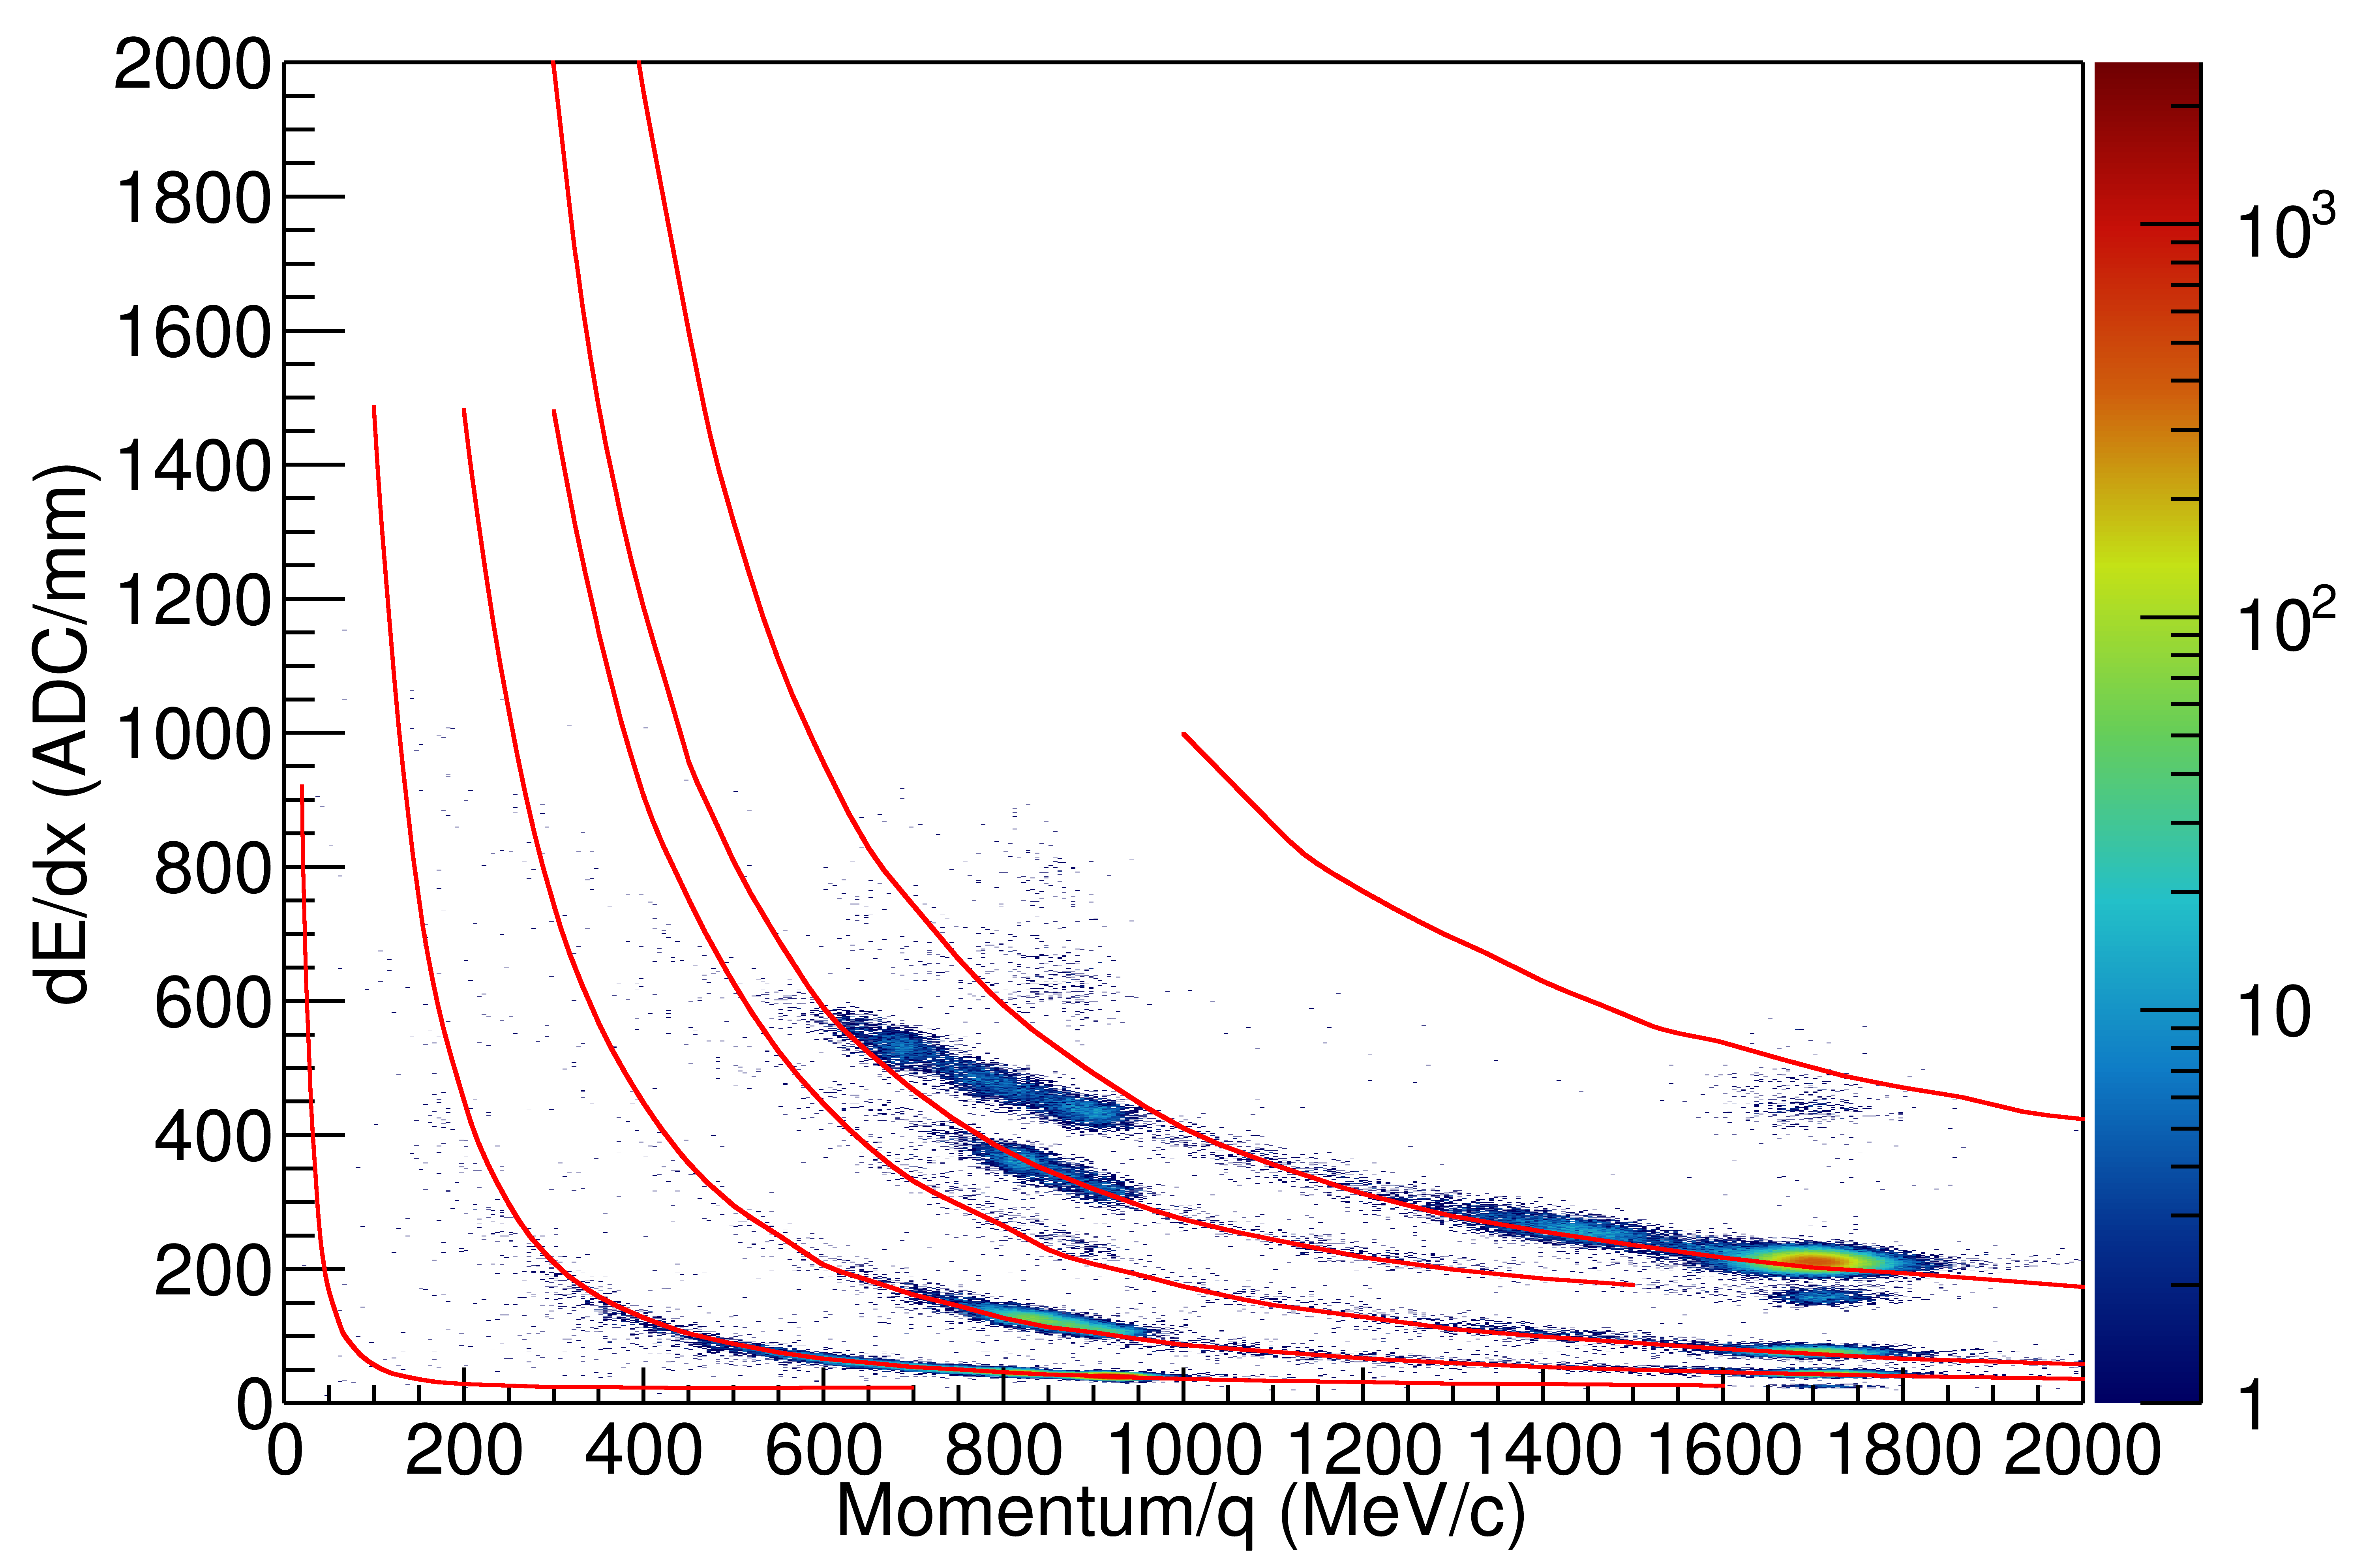
\includegraphics[width=\linewidth]{cocktail_sat.png}
%\caption{Uncorrected cocktail data.}
%\label{fig:cocktail_raw}
%\end{figure}

Looking at the ideal case of the cocktail beam in figures \ref{fig:cocktail_raw} and \ref{fig:cocktail_desat} we note the very clean pronounced PID lines of several particle species. Once can clearly see the three  B$\rho$ settings of the fragment separator leading to three ovals around 1700 and two near 900 [MeV/c/Z]. The tails of the PID lines leading away from these three ovals are resulting from the particle losing its initial energy by passing through the walls and other materials outside the main detector volume, therefore lowering their initial momentum. The red lines are the theoretical PID lines representing the most probable energy loss as given by Geant4 straggling functions after calibration to the experimental data. 

The uncorrected data in figure \ref{fig:cocktail_raw} shows the effects of saturation. It seems the dE/dx values plateau and the PID lines deviate from their theoretical expectations starting around 400 ADC/mm as we also saw previously in figure \ref{fig:lowvshigh_raw}. After applying the desaturation technique we see a stark difference in figures the PID. Most notable is the difference between He and Li particles which suffer the most from saturation. Also a more subtle improvement of the lighter particles, (p,d,t), can also be seen in the PID values at lower momentum.

\begin{figure}[H]	
\begin{overpic}[width=\linewidth]{cocktail_desat.png}
\put(22,15){\contour{white}{\Large p} }
\put(27,20){\contour{white}{\Large d} }
\put(31,25){\contour{white}{\Large t} }
\put(30,31){\contour{white}{\large ${}^{3}$He} }
\put(34,35){\contour{white}{\large ${}^{4}$He} }
\put(60,27){\contour{white}{\large ${}^{6}$Li} }
\end{overpic}
\caption{Corrected (desaturated) cocktail data.}
\label{fig:cocktail_desat}
\end{figure}

%\begin{figure}[H]
%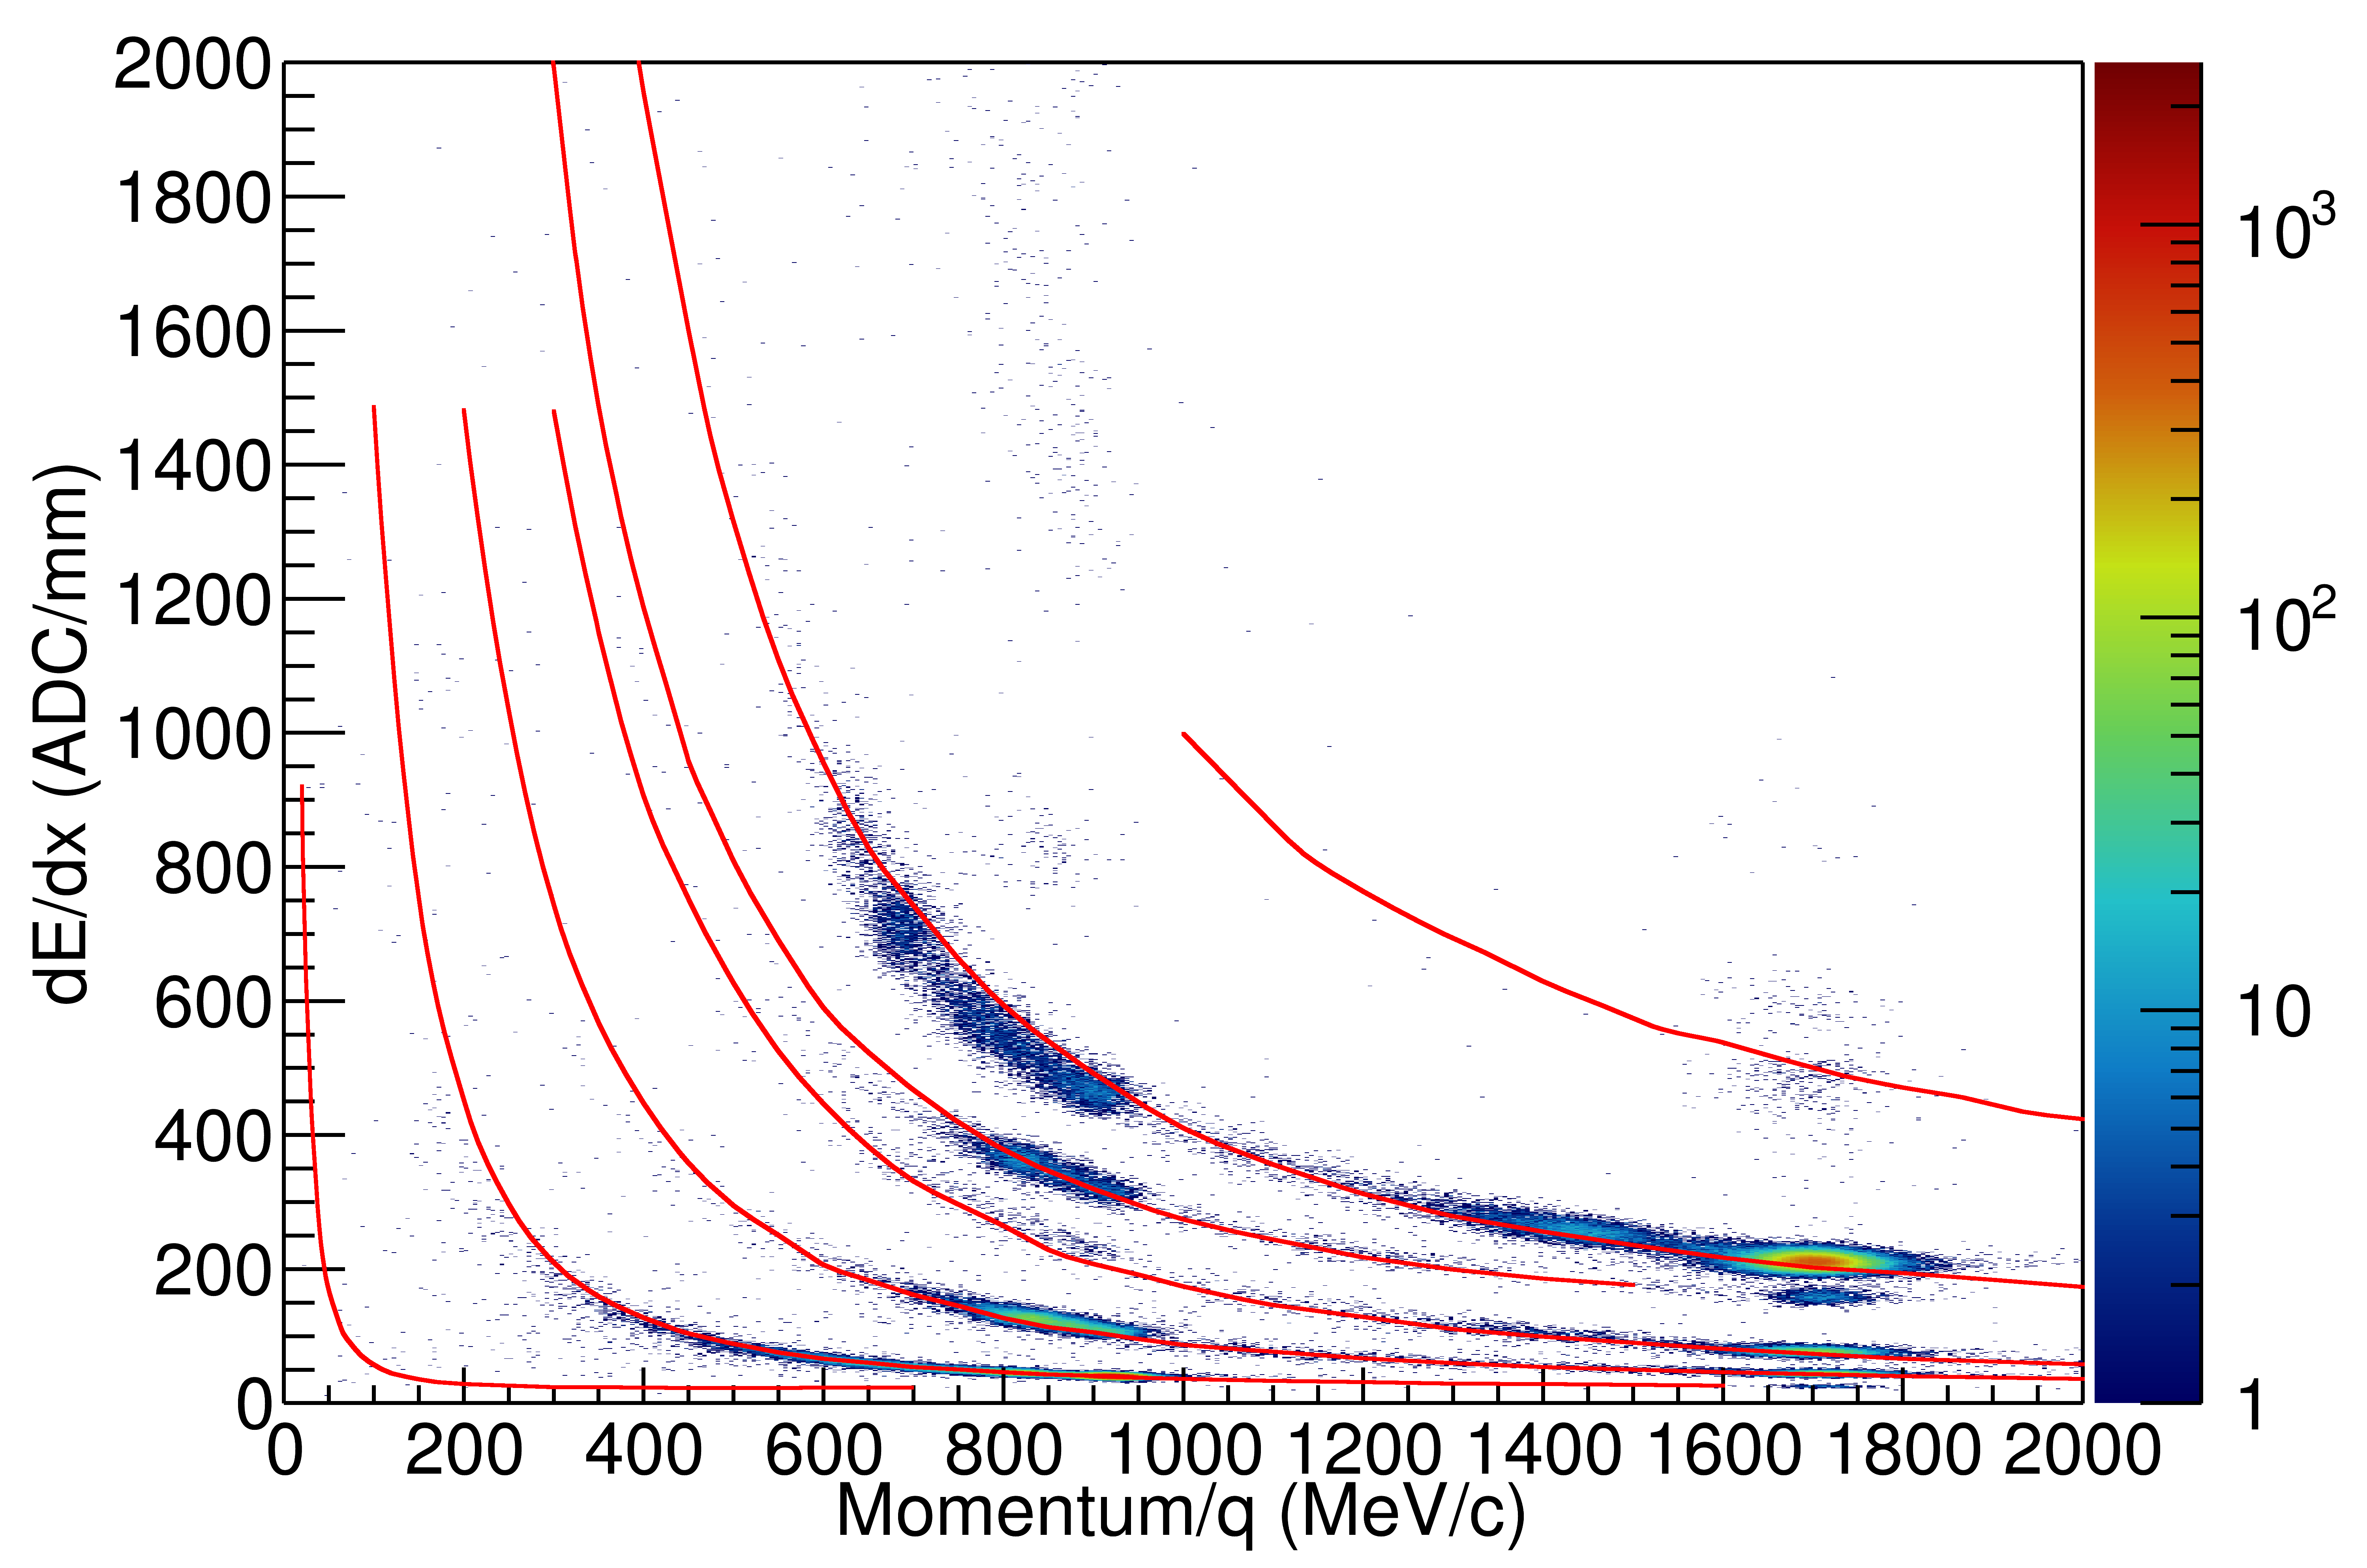
\includegraphics[width=\linewidth]{cocktail_desat.png}
%\caption{Corrected (desaturated) cocktail data.}
%\label{fig:cocktail_desat}
%\end{figure}


 
Looking at the collision data in figures $\ref{fig:data_raw}$ and $\ref{fig:data_desat}$ we also see a similar result. Of course the collision data PID is much less clean than the ideal case of the cocktail beam, nevertheless we can see a similar improvement in the PID lines of the real data when comparing the raw to after the desaturation has been applied. Noted by the fact of the separation of particle species at lower momenta and the separation of the Li species into ${}^{6}$Li and ${}^{7}$Li.

\begin{figure}[H]	
\begin{overpic}[width=\linewidth]{data_sat.png}
\put(22,15){\contour{white}{\Large p} }
\put(27,20){\contour{white}{\Large d} }
\put(31,25){\contour{white}{\Large t} }
\put(30,31){\contour{white}{\large ${}^{3}$He} }
\put(34,35){\contour{white}{\large ${}^{4}$He} }
\put(60,27){\contour{white}{\large ${}^{6}$Li} }
\end{overpic}
\caption{Uncorrected collision data.}
\label{fig:data_raw}
\end{figure}

%\begin{figure}[H]
%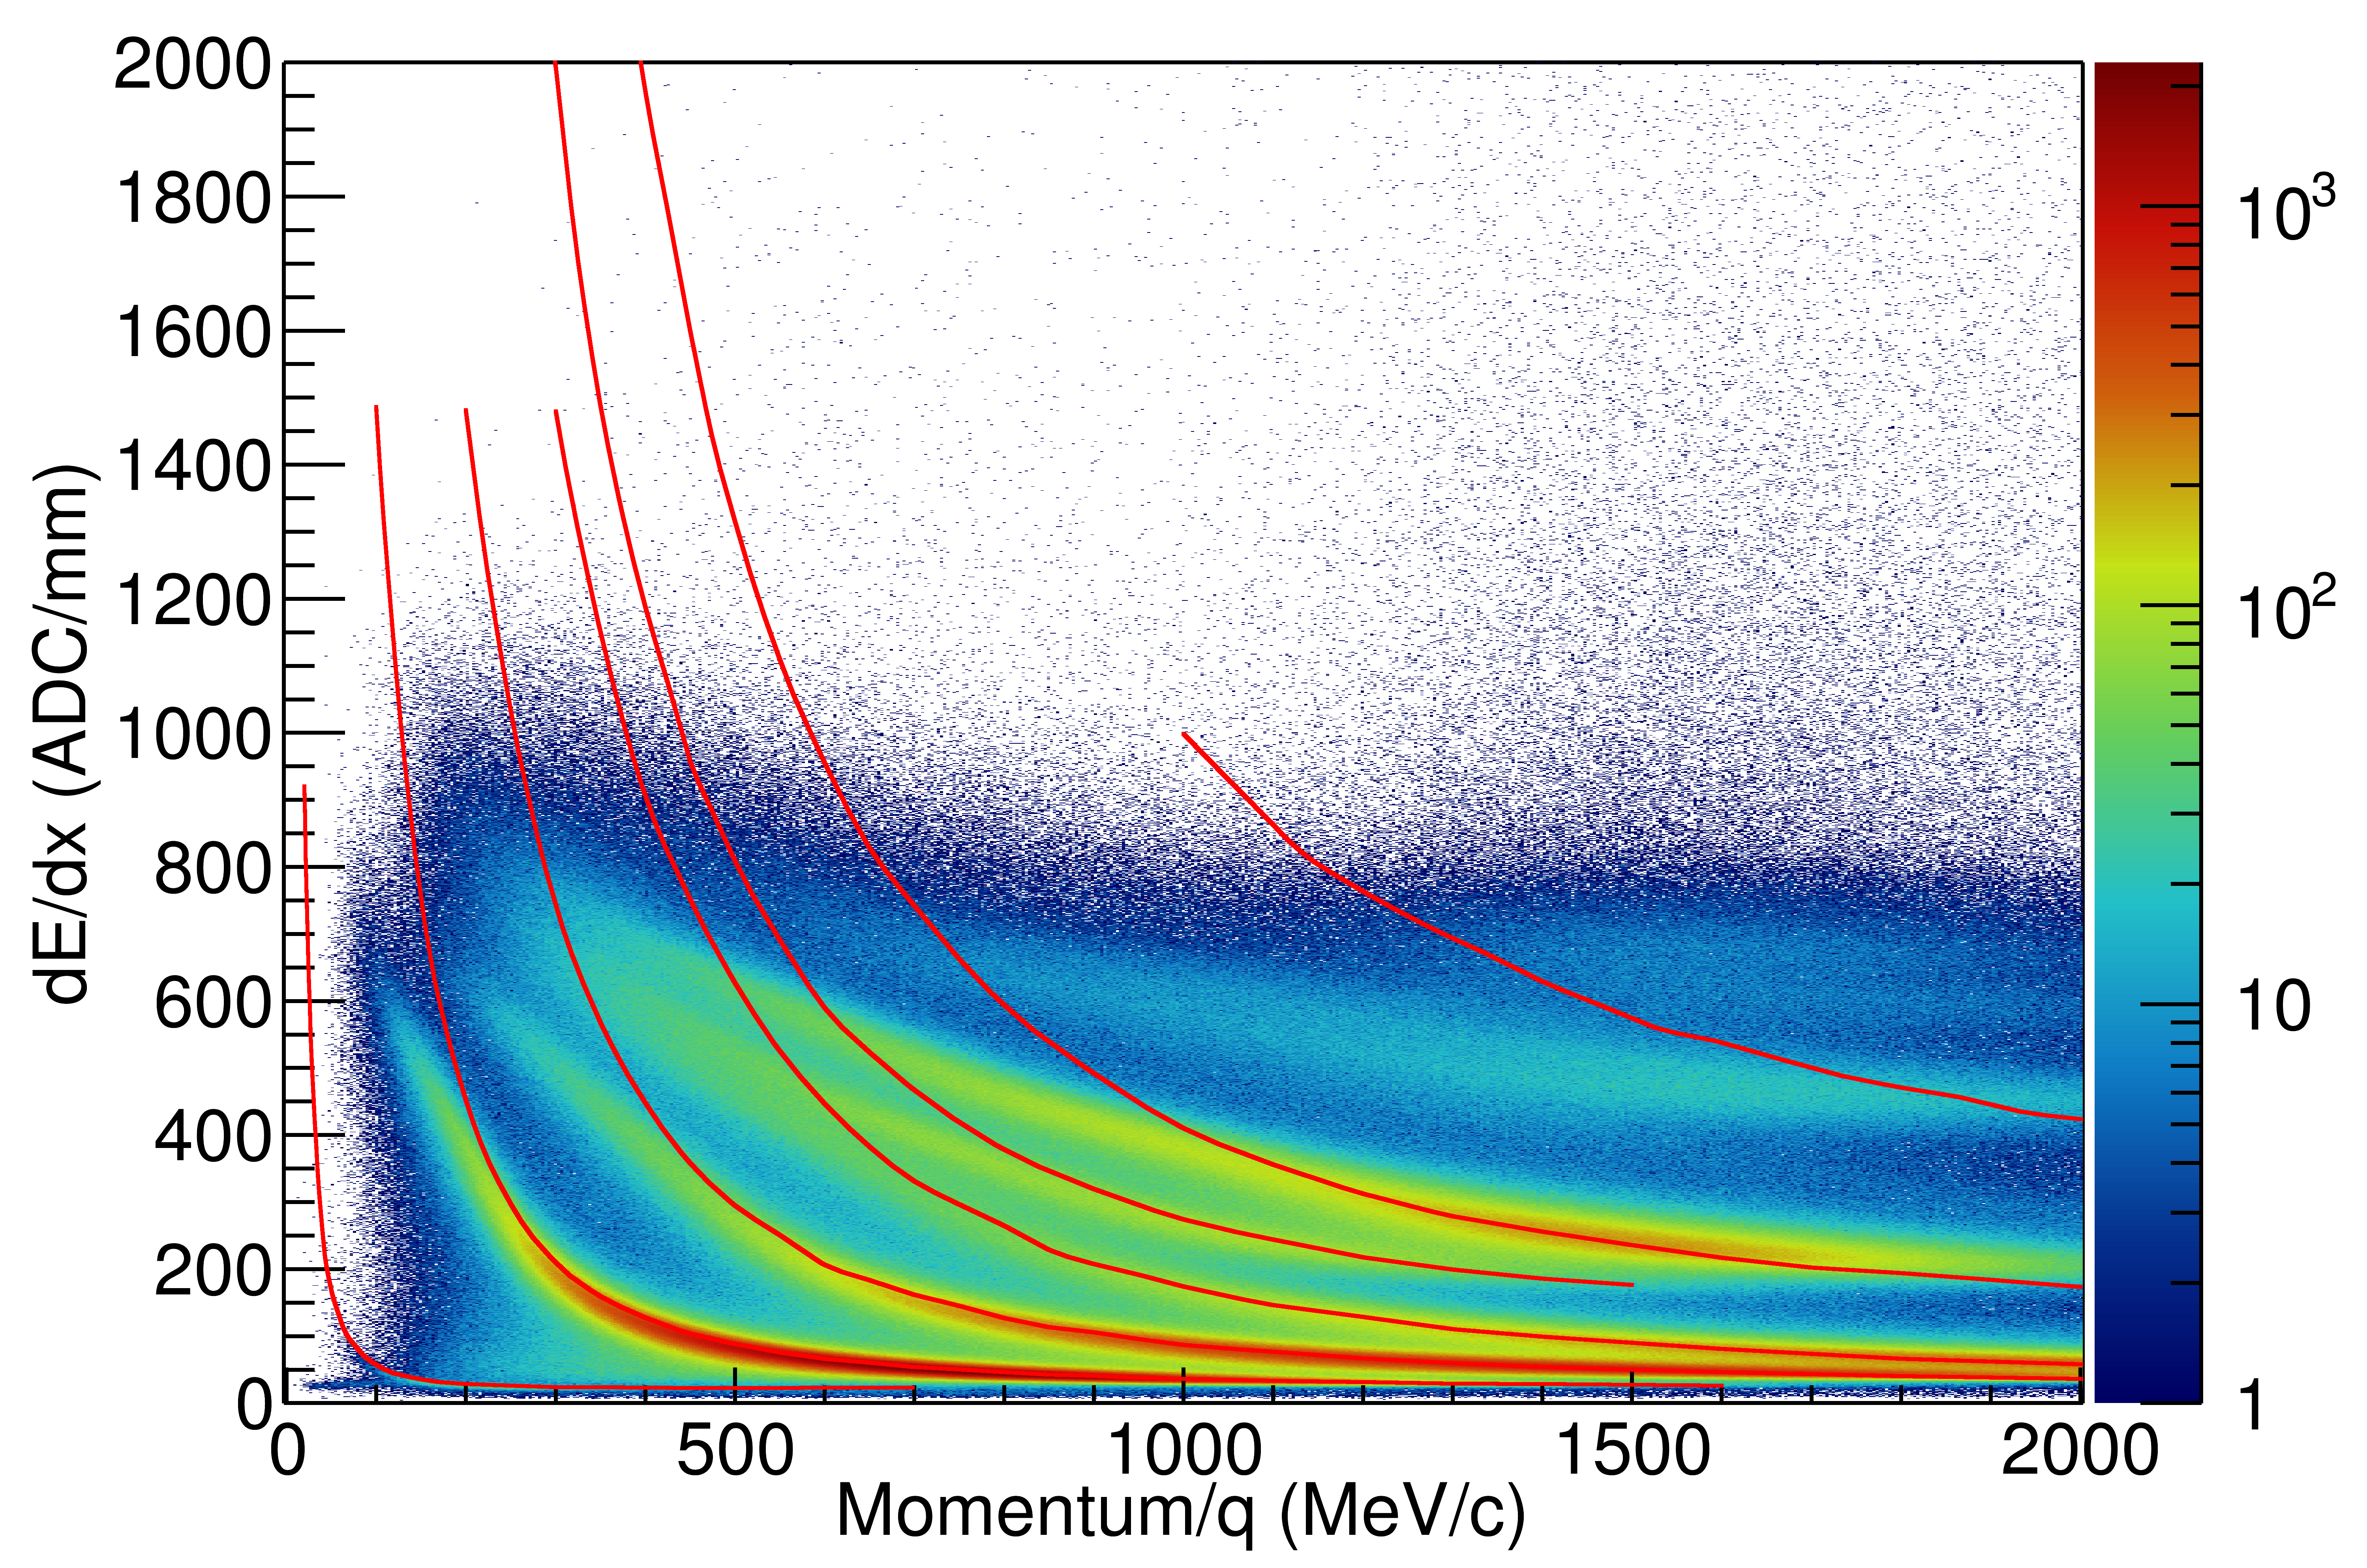
\includegraphics[width=\linewidth]{data_sat.png}
%\caption{Uncorrected collision data.}
%\label{fig:data_raw}
%\end{figure}


\begin{figure}[H]	
\begin{overpic}[width=\linewidth]{data_desat.png}
\put(22,15){\contour{white}{\Large p} }
\put(27,20){\contour{white}{\Large d} }
\put(31,25){\contour{white}{\Large t} }
\put(30,31){\contour{white}{\large ${}^{3}$He} }
\put(34,35){\contour{white}{\large ${}^{4}$He} }
\put(60,27){\contour{white}{\large ${}^{6}$Li} }
\end{overpic}
\caption{Corrected (desaturated) collision data.}
\label{fig:data_desat}
\end{figure}

%\begin{figure}[H]
%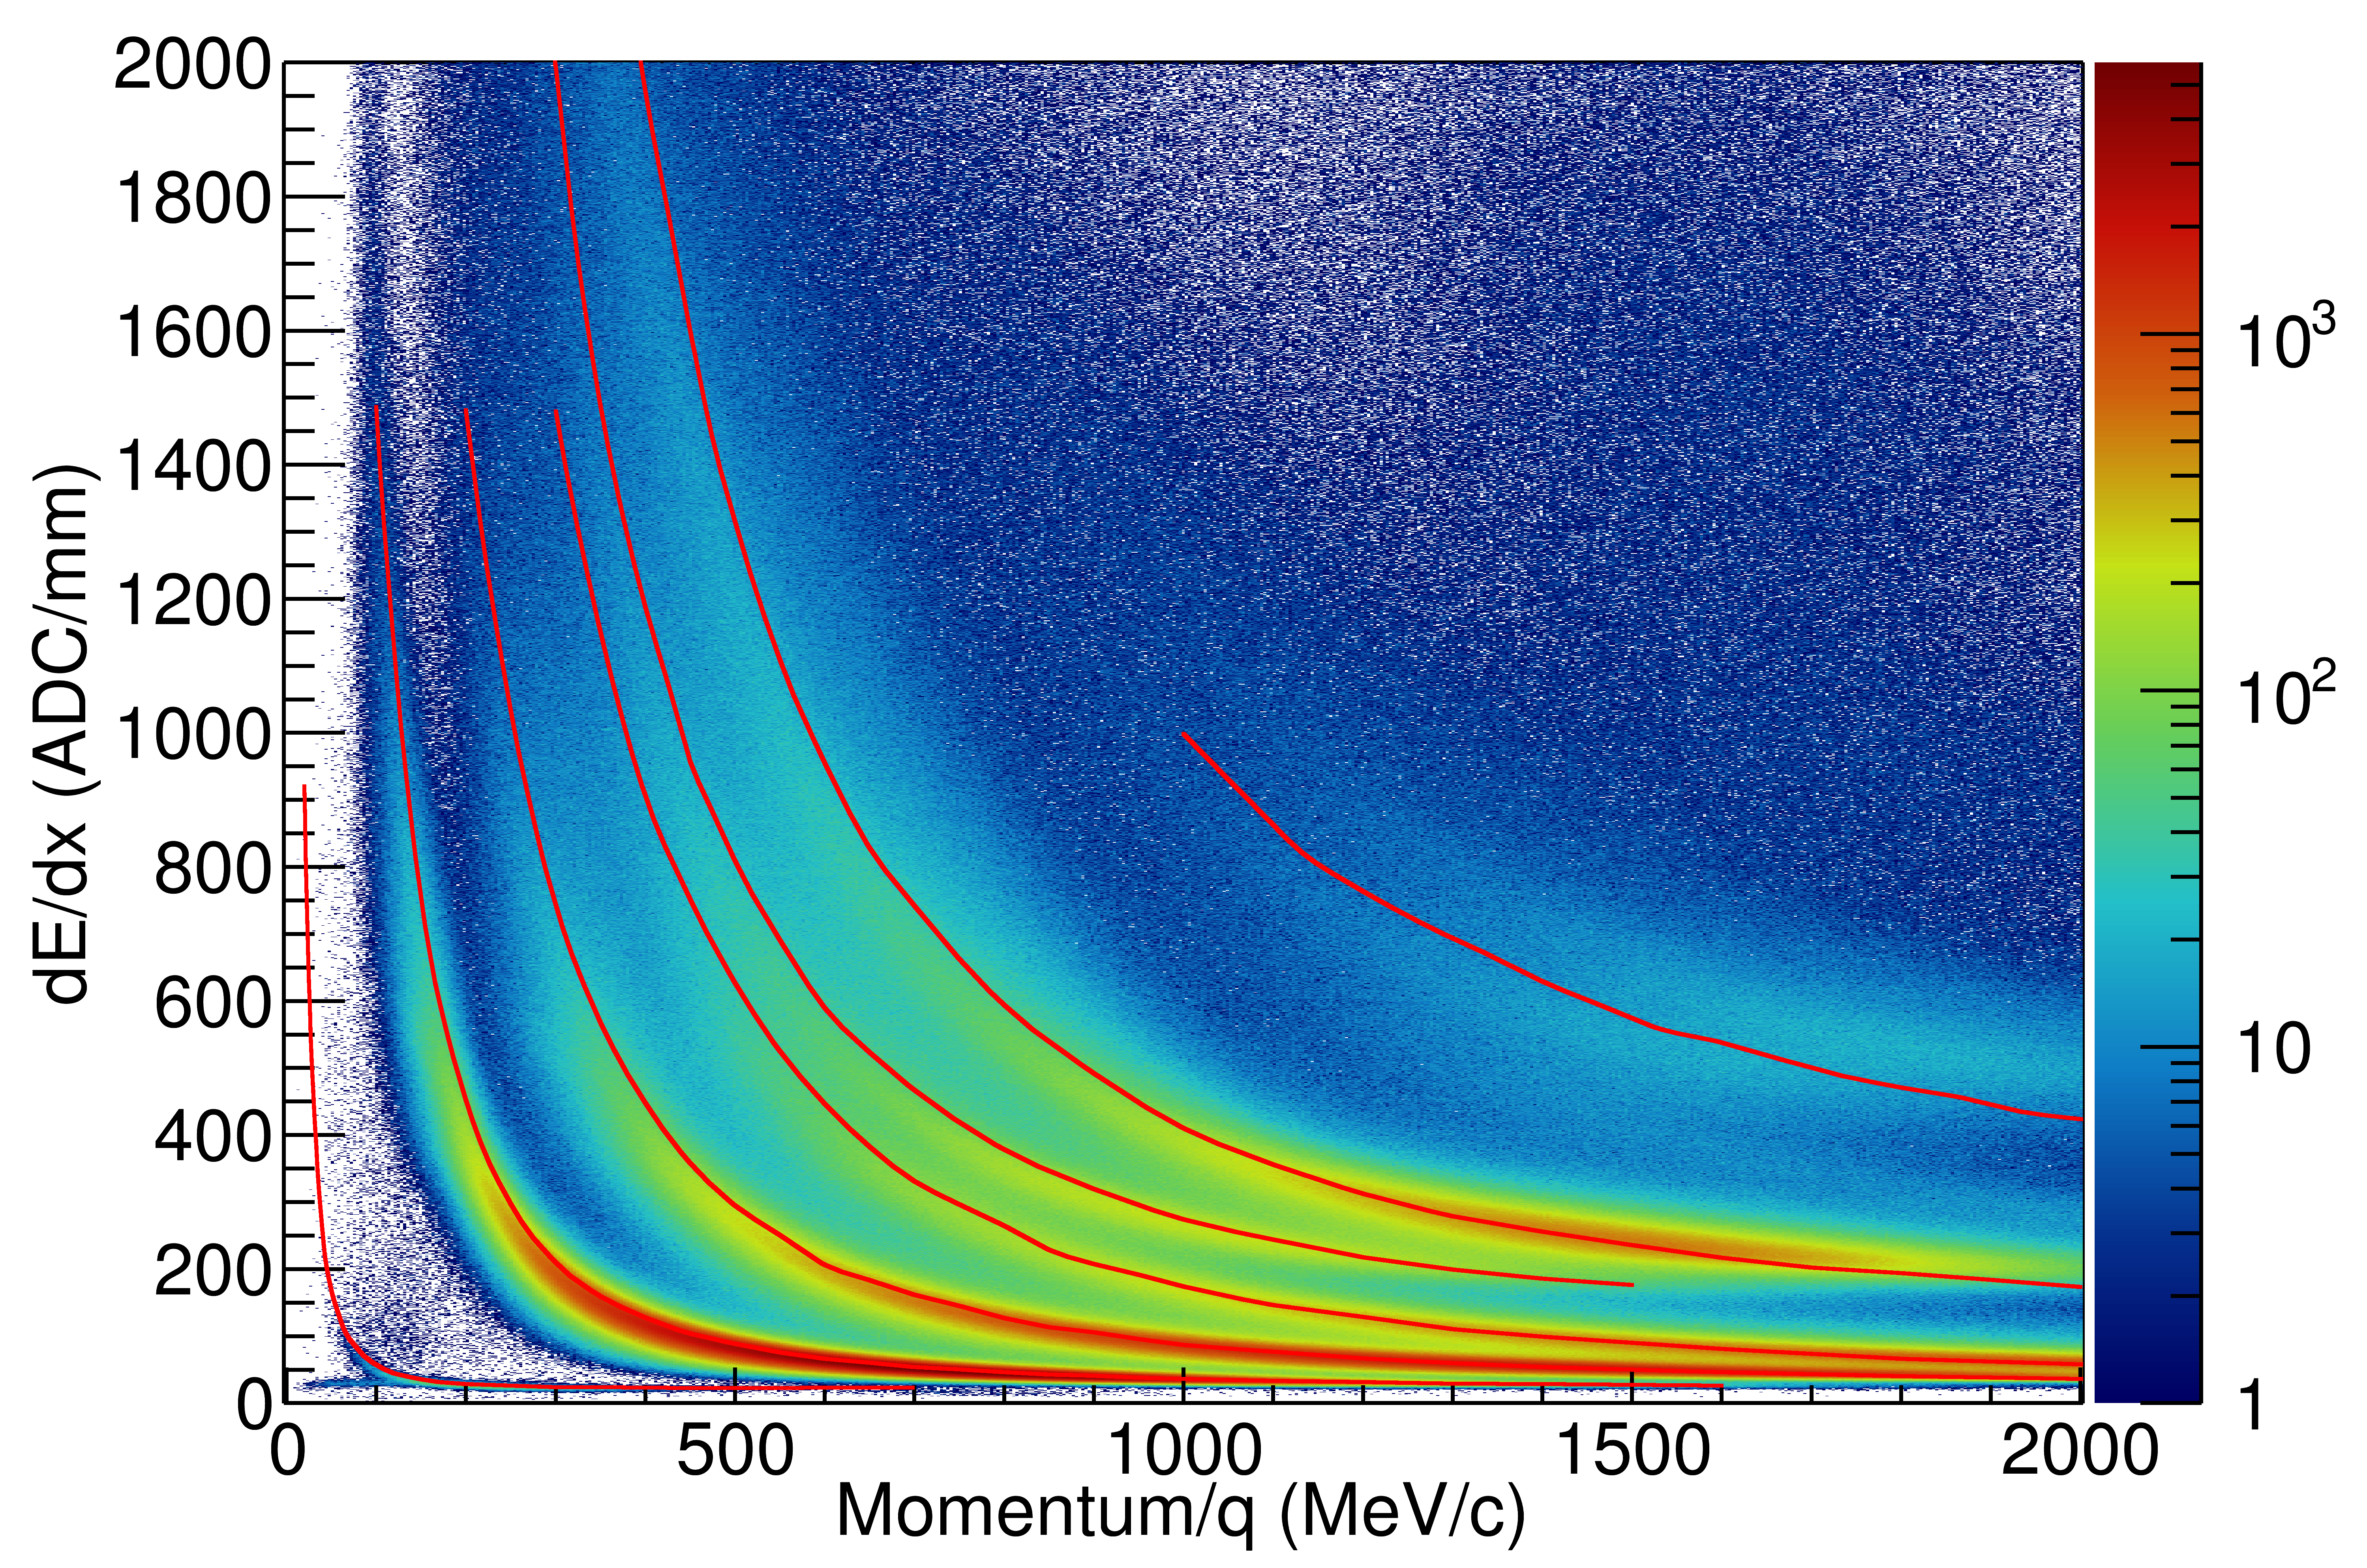
\includegraphics[width=\linewidth]{data_desat.png}
%\caption{Corrected (desaturated) collision data.}
%\label{fig:data_desat}
%\end{figure}


\section{Conclusion}
While saturation reduces dE/dx resolution and even the maximum charge observable inside of a TPC we have shown that some of the saturation is recoverable. By using the knowledge that a TPC's PRF is fixed by the anode wire geometry of the TPC and an experimental PRF can be calculated from unsaturated experimental data. Since the pads must follow this PRF only the pads nearest to the avalanche saturate while the pads further away are not saturated. By applying a simple $\chi^2$ fit to the unsaturated tails of pad distribution, one can recover the saturated pad's charges. 

Looking at the PID lines and also making a direct comparison to some low gain sections of the TPC we were able to extend the dynamic range of our electronics by a factor of about 5x. This improved PID will allow for us to extend the momentum distributions of all species to lower momenta than what was previously available. 

\section*{References}

\bibliography{mybibfile}

\end{document}